\chapter{Bitonic Sort}

\section{Funzionamento generale}

L'algoritmo di \textit{Bitonic Sorting} produce una sequenza ordinata dopo alcune iterazioni di \textit{Bitonic Merge}, che convertono due sequenze bitoniche di grandezza \textit{m} in un'unica sequenza monotona di grandezza \textit{2m}.
La figura \ref{bitonic1} mostra una rete di ordinamento bitonico per 8 valori.

\begin{figure}[h!]
  \centering
  \includegraphics[width=\linewidth]{Images/bitonic1.png}
  \caption{Rete di ordinamento bitonico per 8 valori}
  \label{bitonic1}
\end{figure}

Ogni segmento verticale rappresenta un comparatore a 2 ingressi e 2 uscite e con una sua polarità, il quale svolge un'operazione \textit{Compare and Exchange}. Un comparatore con la freccia verso il basso restituisce il valore più alto alla porta più bassa e viceversa. Un comparatore con la freccia verso l'alto, invece, restituisce il valore più alto alla porta più bassa e viceversa.

\section{Implementazione parallela}

Nella mappatura del \textit{Bitonic Sort} su architetture parallele ogni comparatore è sostituito da una coppia di processori che svolgono un'operazione chiamata \textit{Merge and Split}. Ogni processore è a carico di un numero $n = N / P$ di valori, di cui ne mantiene una lista ordinata durante l'esecuzione. La figura \ref{bitonic2}, ad esempio, mostra l'ordinamento di 16 valori con 4 processori.

\begin{figure}[h!]
  \centering
  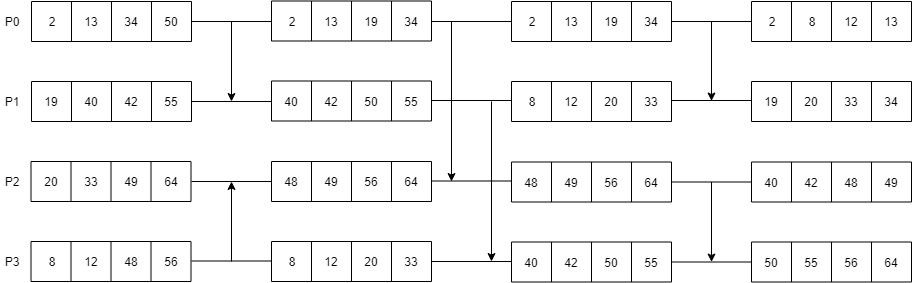
\includegraphics[width=\linewidth]{Images/bitonic2.png}
  \caption{Esempio di rete bitonica su archiettura parallela}
  \label{bitonic2}
\end{figure}

In un'operazione di \textit{Merge and Split}, date in ingresso due sequenze ordinate, esse vengono unite in un'unica sequenza ordinata, che sarà poi sezionata nella sua parte maggiore e parte minore. Ogni processore terrà in memoria solo la parte maggiore (polarità \textit{U}) o minore (polarità \textit{L}) in base alla sua polarità (direzione della freccia), similmente a quanto accadeva nell'operazione \textit{Compare and Exchange}.

L'algoritmo fa in modo che ogni processore mantenga lo stesso numero di dati, quindi bilancia perfettamente il carico di lavoro in ogni ciclo. D'altra parte, se è implementato in un sistema parallelo a memoria distribuita, una grande porzione del tempo è dedicata alle comunicazioni interprocessore. Questo è causato dal fatto che l'algoritmo richiede che ogni processore scambi tutti i suoi dati durante la fase \textit{Merge and Split}.

Per questo in \ref{PaperBitonic} si è cercato di ridurre il numero di dati da scambiare in tali fasi. Invece di inviare tutti i suoi $n$ valori, infatti, ogni processore può inviare solo i dati effettivamente necessari. Dato che, alla fine dell'iterazione, un processore terrà solo una parte del risultato del \textit{merging}, sarà necessario inviare solo le chiavi necessarie a determinare questa lista di $n$ valori. Inizialmente, ogni coppia di processori scambia con l'altro il suo valore minimo se ha polarità U, il suo valore massimo se ha polarità L. Dato che sicuramente il processore con polarità L non terrà i valori che sono maggiori del suo massimo, il processore con polarità U può inviare a quest'ultimo solo i valori minori di tale massimo. Similmente, dato che sicuramente il processore con polarità U non terrà i valori che sono minori del suo minimo, il processore con polarità L può inviare a quest'ultimo solo i valori maggiori di tale minimo. Considerando il valore ricevuto dall'altro processore, vengono quindi inviati solo i valori che effettivamente hanno una possibilità di entrare nella lista alla fine dell'iterazione.

Successivamente, il processore L sceglierà semplicemente i valori più piccoli tra quelli inviati e quelli ricevuti da U e viceversa.

Un esempio dell'intero procedimento può essere visto in figura \ref{mergeAndSplit}.

\begin{figure}[h!]
  \centering
  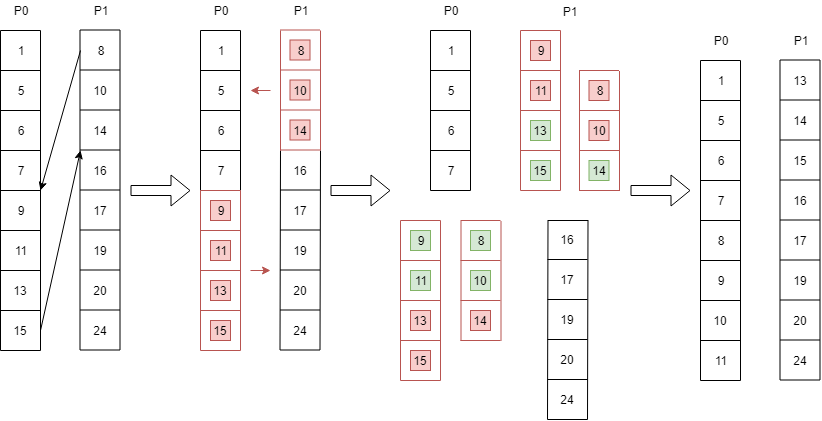
\includegraphics[width=\linewidth]{Images/mergeAndSplit.png}
  \caption{Fase modificata di Merge and Split}
  \label{mergeAndSplit}
\end{figure}

La riduzione del numero di valori da trasferire nel canale di comunicazione si dovrebbe tradurre in un aumento delle prestazioni. La ricerca del valore e la preparazione del buffer da trasferire introducono però operazioni aggiuntive a ogni iterazione. Il vantaggio sussiste, di conseguenza, solo se la taglia del problema rende il risparmio sulla comunicazione maggiore dell'\textit{overhead} introdotto.

\subsection{Descrizione dell'implementazione}

L'implementazione utilizzando \textit{MPI} segue quasi alla lettera il procedimento appena descritto.

Ricevuta la sequenza da ordinare, il processore \textit{MASTER} divide equamente i valori tra tutti i processori.

Dopodiché, ogni processore ordina la lista di valori ricevuta utilizzando l'ordinamento bitonico sequenziale (in \ref{PaperBitonic} venivano invece generate sequenze ordinate direttamente in ogni processore, ma si è deciso di seguire la strada dell'ordinamento per rendere il funzionamento del programma affine a quello del \textit{Quick Sort}, descritto nel prossimo capitolo).

L'implementazione del Bitonic Sort è di tipo iterativo, ottenendo un risparmio in memoria primaria. Per determinare quali sono le coppie su cui si svolge l'operazione di \textit{Compare and Exchange} viene utilizzato il seguente metodo: k seleziona la posizione del bit che determina se la coppia di elementi deve essere scambiata in ordine crescente o decrescente, la variabile j corrisponde alla distanza a cui devono essere gli elementi interessati al \textit{Compare and Exchange}, la variabile i iterata su tutti gli elementi, $i XOR j$ è l'elemento accoppiato a i (cioè l'elemento la cui posizione differisce solo per il bit in posizione $log_2 j$). Viene fatto il confronto solo se $i < ixj$, in modo da non ripetere lo stesso confronto due volte.

Dopo questo passo ogni processore contiene una sequenza ordinata di $n = N / P$ valori, si può quindi procedere con l'algoritmo parallelo descritto precedentemente. 

Per determinare il rango dei processori che devono comunicare viene utilizzato un metodo del tutto simile a quello applicato per l'ordinamento sequenziale. A ogni iterazione i processori accoppiati si mettono in comunicazione e svolgono il processo di \textit{Merge and Split} chiamando la funzione \textit{void mergeAndSplit(int in[], int rank, int r\_min, int r\_max, int num\_keys)}. Il ruolo di ogni processore viene determinando passando il suo rango come parametro in r\_max se ha polarità U o in r\_min altrimenti. Il processore con cui si comunica viene determinando passando il suo rango come parametro in, rispettivamente, r\_min o r\_max.

All'interno di questa funzione ogni processore seguirà una strada diversa in base alla polarità assegnata al suo rango. Le due strade sono simmetriche tra loro e corrispondono a quelle illustrate in figura \ref{mergeAndSplit}.

In base alla polarità ogni processore invia, a questo punto, il suo massimo o minimo al suo compagno. Una volta ricevuto il valore ogni processore esegue una ricerca binaria iterativa per trovare all'interno dei suoi dati il primo valore maggiore o uguale a quello ricevuto, l'indice relativo viene salvato nella variabile $c$.

Vengono quindi preparati i buffer per l'invio dei dati: il processore con polarità L invierà solo i dati da $c$ a $n - 1$, il processore con polarità U quelli da $0$ a $c$.

Una volta ricevuti i dati ogni processore mantiene i valori massimi o minimi presenti nel buffer inviato e in quello ricevuto in base alla sua polarità e li inserisce nel vettore dei suoi valori mantenendone l'ordinamento.

Una volta terminate tutte le iterazioni il processore \textit{MASTER} raccoglie tutti i dati e ottiene quindi la sequenza ordinata che viene restituita al processo chiamante.
